% =============================================================================
\subsection{Construction of the Junction Tree}\label{sec:constructjt}

\begin{frame} 
\mode<presentation>{
    \begin{center} \huge
        \subsecname
    \end{center}
    \begin{center}
	 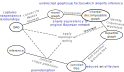
\includegraphics[width=0.8\textwidth]{img/jt_roadmap}%
	\end{center}
}
\end{frame}

\subsubsection{The running intersection property}

\begin{frame}\frametitle{\subsubsecname}
 
    \begin{minipage}{0.5\textwidth}
        \begin{block}{The running intersection property}
            %\small
            All nodes on the path between two 
            cliques, which both contain variable $X$, 
            also contain $X$.
        \end{block} 
    \end{minipage}
    \mode<presentation>{
    \hfill
    \begin{minipage}{0.4\textwidth}
            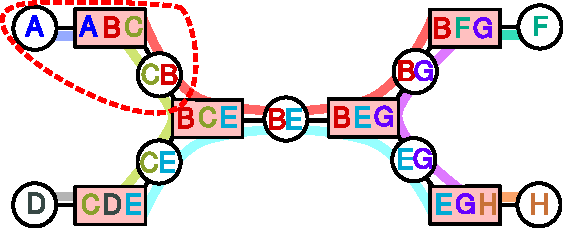
\includegraphics[width=5cm]{img/junction_tree_bipartite}
            \mode<article>{
            \captionof{figure}{The running intersection property}
            }
    \end{minipage}
    }
    \mode<article>{
    
        %\begin{figure}[h]
        {
            \centering
            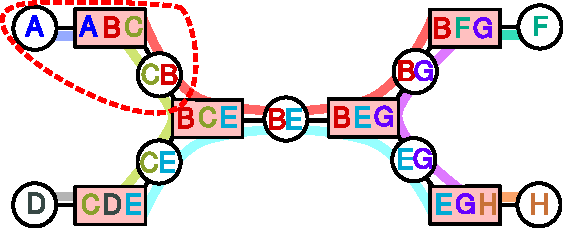
\includegraphics[width=6cm]{img/junction_tree_bipartite}
            \captionof{figure}{The running intersection property}
        }
        %\end{figure}
    }

\only<2>{


\question{Is the following a valid junction tree? \notesonly{ (cf. \figref{fig:isvalidjtexample1})}}\\

        %\begin{figure}[h]
        {
            \centering 
            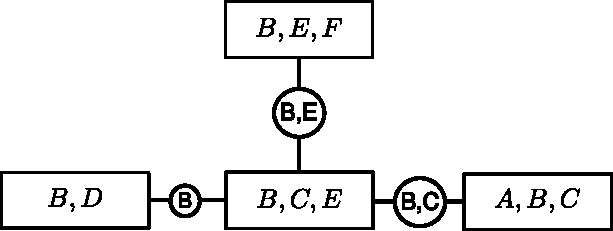
\includegraphics[width=5cm]{img/graph_example_isvalid_junction_tree}
            \mode<article>{
            \captionof{figure}{A valid junction tree}
            }
            \label{fig:isvalidjtexample1}
        }%\end{figure}
}

\only<3,4>{
\question{Which of the following remains a valid junction tree? (irrespective of being useful for exact inference)
 \notesonly{ (cf. \figref{fig:isvalidjtexample2} and \figref{fig:isvalidjtexample3})}}
}

\only<3>{

        %\begin{figure}[h]
        {
            \centering 
            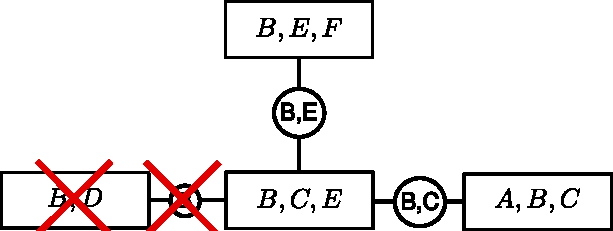
\includegraphics[width=5cm]{img/graph_example_isvalid2_junction_tree}
            \mode<article>{
            \captionof{figure}{This graph remains a valid junction tree}
            }
            \label{fig:isvalidjtexample2}
            }
        %\end{figure}
}
\only<4>{
        %\begin{figure}[h]
        {
            \centering 
            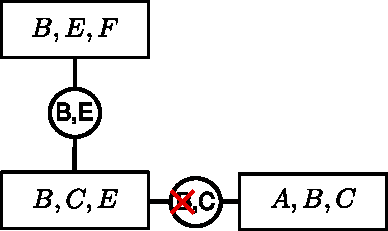
\includegraphics[width=5cm]{img/graph_example_isvalid3_junction_tree}
            \mode<article>{
            \captionof{figure}{This graph no longer qualifies as a junction tree}
            \label{fig:isvalidjtexample3}
            }
            }
        %\end{figure}
}

\end{frame}

\subsection{Identify cliques and separators to form a bipartite graph}

% -----------------------------------------------------------------------------
\begin{frame} \frametitle{\subsecname
}
					\slidesonly{\vspace{5mm}}
				\begin{itemize}
					\item cliques are \underline{maximally} complete subgraphs\\
					(sub-cliques are automatically absorbed)
					\item cliques can be found by elimination \\
					
					\slidesonly{\vspace{10mm}}
					\textbf{Caution: only eliminate a node if it is not part of another clique}
					\slidesonly{\vspace{5mm}}
					%\item sub-cliques $\{A,B\} \subseteq \{A,B,C\}$ are absorbed
					\item requires variable ordering by (\textbf{reverse}) topological sorting: 
						F, D, E, C, B, A
				\end{itemize}
	
	\mode<presentation>{
	\begin{textblock}{}(12,2.5)
		\includegraphics<1->[width=3.cm]{img/graph_example_dag_highlight}
		%\includegraphics<2->[width=3.cm]{img/graph_example_cliques_chordal.jpg}
	\end{textblock}
	}
	
	\mode<article>{
		\begin{figure}[h]
		\centering
		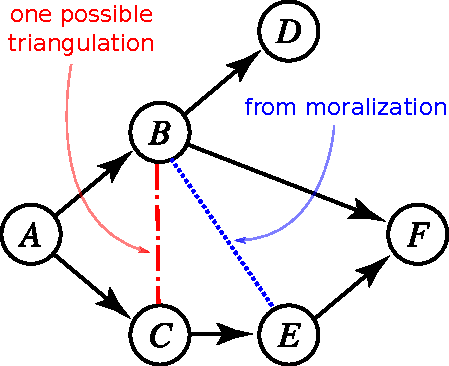
\includegraphics[height=3.5cm]{img/graph_example_dag_highlight}
		\mode<article>{\caption{Example graph from the lecture.}}
		\label{fig:lecexamplecdecompgraph}
		\end{figure}
	}
	
	
	%\begin{textblock}{15}(.5,8.5)
		%\begin{center}
		%\includegraphics<1>[height=3.5cm]{img/graph_example_dag.jpg}
		%\includegraphics<2>[height=3.5cm]{img/graph_example_amoral}
		%\only<2>{\hspace{1cm}}
		%\includegraphics<2>[height=3.5cm]{img/graph_example_moral.png}
		%\includegraphics<3>[height=3.5cm]{img/graph_example_chordal}
		%\only<3>{\hspace{1cm}}
		%\includegraphics<3>[height=3.5cm]{img/graph_example_chordal2}
		%\only<4>{\vspace{7mm}}
		\begin{figure}[h]
		\centering
		\includegraphics<2>[height=2.5cm]{img/graph_example_clique_elimination}
		\mode<article>{
		\caption{Identifying cliques by elimination}
		}
		\end{figure}
		%\includegraphics<3>[height=3.5cm]{img/graph_example_clique_graph}
		%\includegraphics<6>[height=3.5cm]{img/graph_example_junction_tree_v2}
		%\end{center}
	%\end{textblock}
\end{frame}

\subsection{From bipartite graph to junction tree}

\begin{frame} \frametitle{\subsecname
}
		\begin{itemize}		
			\item construct the bipartite graph: 
				\only<1>{ \begin{itemize}
					\item edges weighted by separator size\\ 
						$\rightarrow$ number of nodes within separator
					\item find a {\em maximal spanning tree} 
				\end{itemize}}	
			\item<2-> junction tree for inference
				\only<2>{ \begin{itemize}
					\item maximal spanning tree of the clique graph
					\item data structure for belief propagation
					\item not always unique
				\end{itemize}}			
		\end{itemize}
	
	\mode<presentation>{
	\begin{textblock}{}(12,2.5)
		\includegraphics<1->[width=3cm]{img/graph_example_cliques_chordal.jpg}
	\end{textblock}
	}
	\mode<article>{
		\begin{center}
		%\begin{figure}[h]
		%\centering
		\includegraphics<1>[height=3.5cm]{img/graph_example_cliques_chordal.jpg}
		\mode<article>{\captionof{figure}{Identification of cliques and separators in example graph form \figref{fig:lecexamplecdecompgraph}}}
		\label{fig:lecexamplecliques}
		%\end{figure}
		\end{center}
	}
	
		\begin{center}
		%\begin{figure}[h]
		%\centering
		\includegraphics<1>[height=3.5cm]{img/graph_example_clique_graph}
		\mode<article>{\captionof{figure}{bipartite graph for \figref{fig:lecexamplecliques}}}
		\label{fig:lecbipartitegraph}
		%\end{figure}
		\end{center}
		
		\begin{center}
		%\begin{figure}[h]
		%\centering
		\includegraphics<2>[height=3.5cm]{img/graph_example_junction_tree_v2}
		\mode<article>{\captionof{figure}{junction tree to bipartite graph in \figref{fig:lecbipartitegraph}}}
		%\end{figure}
		\end{center}
		
\end{frame}

\subsection{Inference in a junction tree}

\begin{frame}\frametitle{\subsecname}

\begin{enumerate}
\item clique potentials (non-negative function) for each clique (get definitions from DAG)
\item order initialization according to topological sorting (parent $\rightarrow$ child)
\item add clique potential(s) for observed evidence(s)
\item perform message passing
\item extract marginals from messages
\item perform normalization
\end{enumerate}


\mode<presentation>{
	\begin{center}
		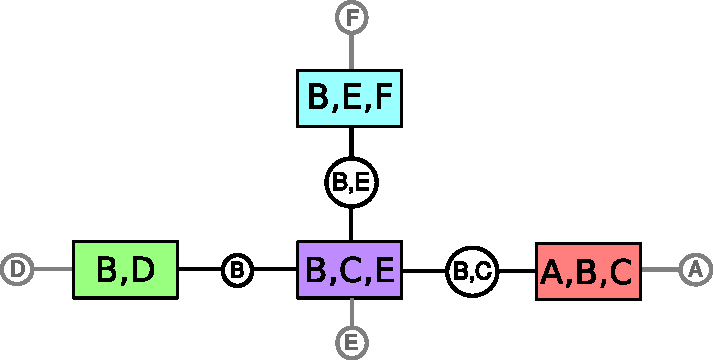
\includegraphics[height=3.5cm]{img/graph_example_junction_tree_v2}
	\end{center}
}

\end{frame}
